\subsection{Выделение признаков}

После проведения предварительной обработки электромиографического (ЭМГ) сигнала необходимо подвергнуть его процедуре извлечения полезной информации. Этот этап является критически важным в процессе разработки системы классификации паттернов. На данном этапе возможно снизить вычислительную сложность, улучшить актуальность обрабатываемых данных и избавиться от излишней информации. Основные особенности сигнала ЭМГ выделяют с помощью временных и частотных характеристик или сверточных нейронных сетей, которые мы рассмотрим подробнее. Важно отметить, что эта процедура играет ключевую роль в дальнейшем анализе и интерпретации сигнала, обеспечивая основу для выделения существенных паттернов и признаков для классификации.

\subsubsection{Временные характеристики}

Функции временной области вычисляются прямо из исходных данных и обладают низкой вычислительной сложностью. Результаты этих функций повышают точность классификации паттернов сигналов ЭМГ. Главным недостатком этих функций является их чувствительность к стационарности сигнала, что приводит к большим изменениям в работе с нестационарными сигналами.

Рассмотрим наиболее эффективные временные характеристики в распознавании сигналов ЭМГ.

\begin{itemize}[parsep=0.4em]
    \setlength\itemsep{0.8em plus 0.2em minus 0.2em}
    \item[1.] Интегральная ЭМГ

        Для получения данной харкатеристики необходимо объеденить сигналы ЭМГ в определенном временном промежутке, размер такого промежутка определяется числом отсчетов $N$. Суммирование ЭМГ сигнала помогает в обнаружении точки активности мышц.

        Данная характеристика описывается следующей формулой:
        \begin{equation}
            \text{G} = \sum\limits_{i=1}^N \bigl|x_i\bigr|,
        \end{equation}
        где $x_i$ -- это измеренный сигнал,\\ \phantom{где} $N$ -- количество заданных временных промежутков.

    \item[2.] Среднее абсолютное значение (MAV)

        Среднее абсолютное значение (MAV) очень схоже с предыдущей характеристикой, однако она менее подвержена воздействию шумов. MAV является одной из наиболее популярных характеристик при анализе сигналов ЭМГ. Данная характеристика необходима в вычислении степени сокращения мышц.

        Среднее абсолютное значение соответствует следующей формуле:
        \begin{equation}
            \text{MAV} = \dfrac{1}{N}\sum\limits_{i=1}^N\bigl|x_i\bigr|,
        \end{equation}
        где $x_i$ -- это измеренный сигнал,\\ \phantom{где} $N$ -- количество заданных временных промежутков.

    \item[3.] Среднеквадратичное значение (RMS)

        RMS можно охарактеризовать как регистрацию постоянного мышечного услилия. Данная характеристика ищется по следующей формуле:
        \begin{equation}
            \text{RMS} = \sqrt{\dfrac{1}{N}\sum\limits_{i=1}^Nx_i^2},
        \end{equation}
        где $x_i$ -- это измеренный сигнал,\\ \phantom{где} $N$ -- количество заданных временных промежутков.

    \item[4.] Длина волны (WL)

        Длина волны (WL) – это мера комплексности сигнала, являющаяся постепенно накапливающейся суммой разностей каждого временного сегмента. Эта характеристика определяется формулой:
        \begin{equation}
            \text{WL} = \sum\limits_{i=1}^{N-1}\bigl|x_{i+1}-x_i\bigr|,
        \end{equation}
        где $x_i$ -- это измеренный сигнал,\\ \phantom{где} $N$ -- количество заданных временных промежутков.

    \item[5.] Сумма квадратов (SSI)

        Другое название данной функции – суммирование элементарных площадей. Данный параметр интерпретируется как мера энергии сигнала. Для вычисления этой характеристики суммируются квадраты значений амплитуды ЭМГ сигнала и вычисляется по формуле:
        \begin{equation}
            \text{SSI} = \sum\limits_{i}^N\bigl|x_i^2\bigr|,
        \end{equation}
        где $x_i$ -- это измеренный сигнал,\\ \phantom{где} $N$ -- количество заданных временных промежутков.

    \item[6.] Оценка дисперсии сигнала (VAR)

        Дисперсия определяется как среднеквадратическое значение отклонения сигнала, так как среднее значение ЭМГ сигнала близко к нулю. Данная характеристика имеет смысл мощности сигнала. Таким образом дисперсия сигнала ЭМГ может вычислена следующим способом
        \begin{equation}
            \text{VAR} = \dfrac{1}{N}\sum\limits_{i=1}^N\bigl(x_i-\bar{x}\bigr)^2;\hspace{0.5cm}\bar{x}\approx 0,
        \end{equation}
        где $x_i$ -- это измеренный сигнал,\\ \phantom{где} $N$ -- количество заданных временных промежутков,\\ \phantom{где} $\bar{x}$ -- математическое ожидание (среднее значение).

    \item[7.] Изменение знака наклона (SSC)

        SSC – функция, которая позволяет определять положительное и отрицательное изменение знака наклона, рассчитывается в течение трех периодов.
        \begin{equation}
            \text{SSC} = \sum\limits_{i}^{N} f\bigl[(x_i-x_{i-1})\times(x_i-x_{i+1})\bigr],
        \end{equation}
        \begin{equation}
            f(x)=
            \begin{cases}
                1, & \text{если } x \geq \Theta\\
                0, & \text{в остальных случаях}
            \end{cases},
        \end{equation}
        где $x_i$ -- это измеренный сигнал,\\ \phantom{где} $N$ -- количество заданных временных промежутков,\\ \phantom{где} $\Theta$ -- пороговое значение. 

    \item[8.] Пересечение нулевой линии (ZC)

        ZC – функция, отражающая сколько раз сигнал пересек нулевую линию с заданным пороговым значением. Данная характеристика вычисляется по формуле:
        \begin{equation}
            \text{ZC} = \sum\limits_{i=1}^{N-1} \text{sgn}(x_i,x_{i+1}),
        \end{equation}
        \begin{equation}
            \text{sgn}(x_i,x_{i+1}) =
            \begin{cases}
                1, & \text{если } x_i\times x_{i+1}<0 \text{ и } x_i-x_{i+1} \geq \Theta\\ 
                0, & \text{в остальных случаях}
            \end{cases},
        \end{equation}
        где $x_i$ -- это измеренный сигнал,\\ \phantom{где} $N$ -- количество заданных временных промежутков,\\ \phantom{где} $\Theta$ -- пороговое значение. 

\end{itemize}

\subsubsection{Частотные характеристики}

Функции, которые рассматриваются в данном разделе, получаются с помощью применения преобразования Фурье и анализируются при помощи метода периодограммы. В отличие от функций во временной области, функции в частотной области отображают изменения сигнала в определенном диапазоне частот. Основные характеристики в частотной области включают спектральную плотность мощности, среднюю спектральную плотность мощности, медианную частоту и среднюю частоту \cite{bib:feature:1}.

Преобразование Фурье (FT) использует интегральное преобразование для представления исходного сигнала в виде базисных функций, выраженных через мнимые экспоненты с различными частотами, амплитудами и фазами. Это позволяет представить исходную функцию как сумму синусоид с различными характеристиками.

Однако преобразование Фурье не дает информации о том, как меняется частотный состав сигнала во времени. Для анализа этих изменений необходимо разбить сигнал на временные сегменты и вычислить спектр для каждого отрезка. Для этой цели используется кратковременное преобразование Фурье (STFT).

STFT определяется следующей формулой:
\begin{equation}
    \text{STFT}(k,l) = \sum\limits_{n=0}^{N-1}h(n)x(n+lL)e^{-i\omega_k n},
\end{equation}
где $x(t)$ -- входной сигнал,\\ \phantom{где} $h(n)$ -- оконная функция,\\ \phantom{где} $k=\overline{0,N-1}$ -- частотный индекс,\\ \phantom{где} $L$ -- временной шаг анализа (расстояние между соседними фреймами),\\ \phantom{где} $l$ -- номер фрейма анализа.

Периодограмма является функцией от частоты, используемой для оценки спектральной плотности. Её применение позволяет идентифицировать различные компоненты сигнала ЭМГ, включая постоянную, сезонную и случайную составляющие. Этот метод также способствует обобщенному анализу структуры временного ряда, который представляет собой последовательность данных, собранных с датчиков через определенные временные интервалы.

Рассмотрим наиболее эффективные частотные характеристики в распознавании сигналов ЭМГ \cite{bib:feature:2}.

\begin{itemize}[parsep=0.4em]
    \setlength\itemsep{0.8em plus 0.2em minus 0.2em}
    \item[1.] Пиковая частота (PF)

        Пиковая частота – это частота, на которой достигается максимальная мощность в спектре. Данная характеристика определяется следующим образом:
        \begin{equation}
            \text{PF} = \text{max}(P_j);\hspace{0.5cm} j=\overline{1,N},
        \end{equation}
        где $P_j$ -- спектр мощности сигнала,\\ \phantom{где} $N$ -- количество заданных временных промежутков.

    \item[2.] Средняя частота (MNF)


        Средняя частота рассчитывается как сумма произведений спектра мощности ЭМГ на частоту, разделенная на суммарную мощность спектра. MNF также называют центральной частотой или спектральным центром тяжести.

        Связь между частотным контентом и рекрутированием основана на том, что средняя частота спектра мощности отображает скорость распространения электрических нервных импульсов по мышечным волокнам.

        MPF имеет низкую эффективность в оценке скорости импульсов двигательных единиц, но при этом может использоваться для изучения качественного состава рекрутируемых волокон.
        \begin{equation}
            \text{MNF} = \dfrac{\sum\limits_{j=1}^N f_jP_j}{\sum\limits_{j=1}^N P_j},
        \end{equation} 
        где $P_j$ -- спектр мощности сигнала,\\ \phantom{где} $f_j$ -- частота сигнала,\\ \phantom{где} $N$ -- количество заданных временных промежутков.

    \item[3.] Средний спектр мощности (MPF)
        \begin{equation}
            \text{MPF} = \sum\limits_{j=1}^N\dfrac{P_j}{N},
        \end{equation}
        где $P_j$ -- спектр мощности сигнала,\\ \phantom{где} $N$ -- количество заданных временных промежутков.

    \item[4.] Общий спектр мощности (TPS)

        Общий спектр мощности является совокупностью всех спектров мощности в исследуемом сигнале и является спектральным моментом нулевого порядка. TPS определяется по следующей формуле
        \begin{equation}
            \text{TPS} = \sum\limits_{j=1}^N P_j = \text{SM}_0.
        \end{equation}

        Спектральный момент ($\text{SM}_i$) порядка $i$ создает новую функцию на основе спектра мощности и определяется как
        \begin{equation}
            \text{SM}_n = \sum\limits_{j=1}^N P_j f_j^n;\hspace{0.5cm} n=\overline{1,n},
        \end{equation}
        где $P_j$ -- спектр мощности сигнала,\\ \phantom{где} $f_j$ -- частота сигнала,\\ \phantom{где} $N$ -- количество заданных временных промежутков.

    \item[5.] Отношение частот (FR)

        \begin{equation}
            \text{FR} = \sum\limits_{j=\text{LLC}}^\text{ULC} P_j - \sum\limits_{j=\text{LHC}}^\text{UHC} P_j,
        \end{equation}
        где $P_j$ -- спектр мощности сигнала,\\ \phantom{где} $\text{ULC}$ и $\text{LLC}$ -- верхняя и нижняя граница низкой частоты,\\ \phantom{где} $\text{UHC}$ и $\text{LHC}$ -- верхняя и нижняя границы высокой частоты.
    
    \newpage
    \item[6.] Оценка дисперсии центральной частоты (VCF)

        \begin{equation}
            \text{VCF} = \dfrac{1}{\text{SM}_0}\sum\limits_{j=1}^N P_j\bigl(f_j-f_c\bigr)^2 = \dfrac{\text{SM}_2}{\text{SM}_0} - \left(\dfrac{\text{SM}_1}{\text{SM}_0}\right)^2,
        \end{equation}
        где $P_j$ -- спектр мощности сигнала,\\ \phantom{где} $f_j$ -- частота сигнала,\\ \phantom{где} $N$ -- количество заданных временных промежутков,\\ \phantom{где} $\text{SM}_i$ -- спектральный момент.

    \item[7.] Медианная частота (MDF)

        Медианная частота -- это разделение двух равных по амплитуде спектров.
        \begin{equation}
            \sum\limits_{j=1}^\text{MDF}P_j=\sum\limits_{j=\text{MDF}}^N=\dfrac{1}{2}\sum\limits_{j=1}^N P_j,
        \end{equation}
        где $P_j$ -- спектр мощности сигнала,\\ \phantom{где} $N$ -- количество заданных временных промежутков.

\end{itemize}


\subsubsection{Сверточные нейронные сети}

Рассмотрим сверточные нейронные сети (CNN) для выделения признаков ЭМГ сигналов. Сети такого вида показали достаточно хорошие результаты при распознавании изображений. Такая особенность CNN позволяет рассматривать не каждый сигнал по отдельности, а все вместе как будто это изображение. В дальнейшем будем считать, что совокупность полученных от разных датчиков данных в одно и тоже время является изображением. Одним из важных преимуществ данной реализации заключается в устойчивости к изменениям масштаба и смещениям изображения.

Основное различие сверточных нейронных сетей от временных и частотных методов заключается в их способности автоматически и эффективно выделять ключевые признаки из изображений без необходимости ручного извлечения характеристик, что также приводит к их постоянному улучшению в процессе обучения.

Архитектура CNN базируется на сверточных слоях, ответственных за начальное извлечение признаков из входных данных с помощью фильтров - небольших матриц с весами. Применение фильтра к изображению основано на математической операции, известной как свертка.

На рисунке \ref{conv_work} показана работа свертки. Фильтр перемещается по всему изображению с определенным шагом (страйдом), умножая веса фильтра на соответствующие значения изображения на каждом этапе, за последующим суммированием. Результатом этой операции является формирование карты признаков, отображающей степень соответствия фильтра каждому локальному участку изображения. Для обеспечения анализа признаков по всему изображению, включая его края, и сохранения пространственного размера карты признаков часто используется паддинг - добавление пикселей вокруг начального изображения.

\addimgh{conv_work}{1}{Работа свертки}{conv_work}

Представим данную операцию на математическом языке. Допустим входным изображением является матрица $I$, а фильтром -- матрица $F$, то свертка в позиции $(i,j)$ вычисляются следующим образом
\begin{equation}
    C(i,j) = \sum\limits_{u=0}^{m-1}\sum\limits_{v=0}^{n-1}I(i+u,j+v)\times F(u,v).
\end{equation}
При этом картка признаков собирается из элементов $C(i,j)$.

При проектировании сверточных нейронных сетей возникает множество трудностей. Одной из таких является то, что в попытке улучшить качесто модели путем увеличения слоев в сети появляется проблема исчезающего градиента \cite{bib:gradient:1}. Она заключается в том, что по мере распространения градиента обратно к начальным слоям он может становиться чрезвычайно малым из-за многократного умножения. Это в свою очередь может привести к быстрому снижению эффективности. Для решения появившейся проблемы используют две популярные архитектуры сверточных нейронных сетей: ResNet и DenseNet. Рассмотрим их более подробно.

\subsubsection{Архитектура ResNet}

Residual Networks (ResNet) – это нейронная сеть, решающая проблему затухающего градиента. Благодаря этому стало возможно успешно обучать глубокие сети с более чем 150 соями. Данная архитектура была разработана исследователями Microsoft Research в 2015 году.

В ResNet была введена концепция, называемая остаточными боками. В ней используются пропускные соединения, которые соединяют слои с другими слоями, при этом пропускают некоторые слои между ними. Повторные соединения определяются путем объединения остаточных блоков вместе. Описанная архитектура изображена на рисунке \ref{resnet}.

\addimgh{resnet}{0.8}{Остаточный блок}{resnet}

Основная идея данного подхода заключается в том, что такое построение архитектуры позволяет пропускать уровни, ухудшающие эффективность модели. Именно поэтому получается обучать довольно глубокие нейронные сети, не обращая внимание на проблему затухающего градиента.

На рисунке \ref{analis_plain_resnet} показаны результаты обучения 18-ти и 34-х уровневых сетей обычных сверточных нейронных сетей и архитектуры ResNet. ResNet показывает лучшие результаты при большей глубине сети.

\subsubsection{Архитектура DenseNet}

Плотно связанные сверточные сети (DenseNet) – это архитектура сверточной нейронной сети с прямой связью (CNN), которая связывает каждый уровень с любым другим уровнем. Это позволяет сети более эффективно обучаться за счет повторного использования функций, следовательно, уменьшая количество параметров и улучшая градиентный поток во время обучения.

Архитектура DenseNet, изображенная на рисунке \ref{densenet}, основана на простом и базовом принципе: путем объединения карт объектов всех предыдущих слоев плотный блок позволяет каждому слою получить доступ к объектам всех предыдущих уровней. В классических CNN каждый слой имеет доступ только к характеристикам слоя, непосредственно перед ним.

\vspace{1em}
\begin{figure}
	\centering
	\begin{subfigure}{0.45\linewidth}
		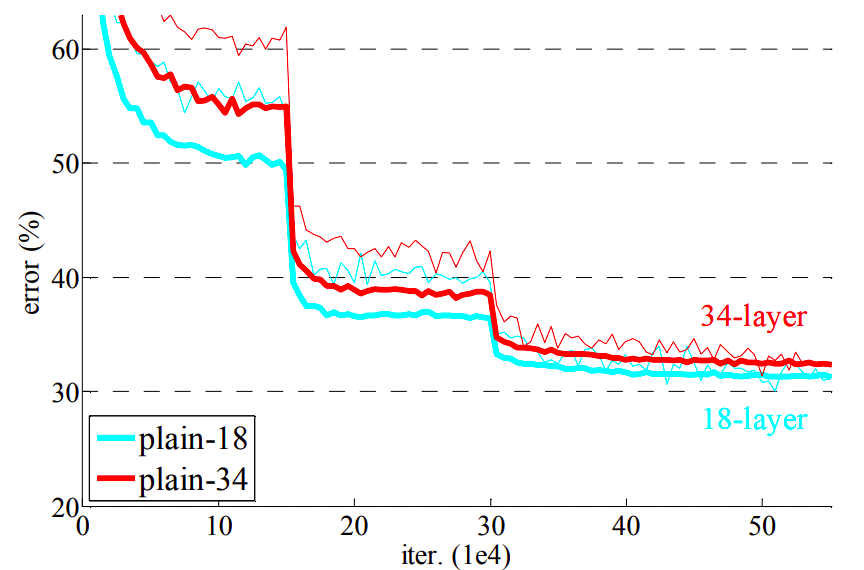
\includegraphics[width=\linewidth]{result_plain}
		\caption{Обычная сверточная сеть}
	\end{subfigure}
    \hfill
	\begin{subfigure}{0.45\linewidth}
		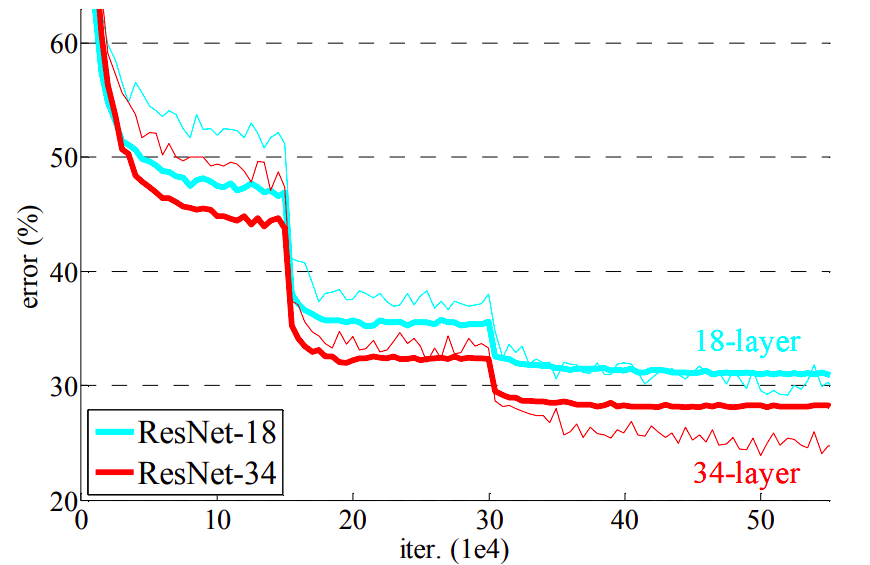
\includegraphics[width=\linewidth]{result_resnet}
		\caption{Архитектура ResNet}
	\end{subfigure}
	\caption{Обучение сверточных сетей}
	\label{analis_plain_resnet}
\end{figure}

DenseNet состоит из переходных слоев и плотных блоков. Каждый сверточный слой внутри плотного блока связан с любым другим слоем внутри блока. Это достигается путем соединения выходных данных каждого слоя со входными данными следующего слоя, создавая «короткую» ссылку. Переходные слои минимизируют размер карт объектов в плотных блоках, что позволяет сети эффективно расти.

Данная нейронная сеть показывает очень хорошие результаты при обучении и является улучшенной версией ResNet. Однако для обучения DenseNet требуются огромные вычислительные затраты, из-за этого данную архитектуру нечасто используют.

\addimgh{densenet}{0.75}{Архитектура DenseNet}{densenet}
